\documentclass[12pt]{article}
\usepackage{sbc-template}
\usepackage{graphicx,url,hyperref}
\usepackage[utf8]{inputenc}
\usepackage[english]{babel}
\usepackage{amsmath,amssymb,amsfonts,amsthm}
\usepackage{algorithm,algpseudocode}
\usepackage{color}
\sloppy

\DeclareMathOperator*{\scope}{scope}
\DeclareMathOperator*{\ch}{ch}
\DeclareMathOperator*{\dagroot}{root}

\algnewcommand{\LineComment}[1]{\State \(\triangleright\) #1}
\algnewcommand{\Input}[1]{\State \textbf{Input:} #1}
\algnewcommand{\Output}[1]{\State \textbf{Output:} #1}

\title{Tractable Mode-Finding in\\Sum-Product Networks with Gaussian Leaves}

\author{Tiago Madeira\inst{1}, Denis Deratani Mauá\inst{1}}

\address{Institute of Mathematics and Statistics -- University of São Paulo (USP)
  \email{\{madeira,ddm\}@ime.usp.br}
}

\begin{document} 

\maketitle

\begin{abstract}
In this work, we leverage the relation between Sum-Product Networks (SPNs) and Gaussian mixtures to propose an algorithm that adapts the Expectation-Maximization method to efficiently find the modes of SPNs with Gaussian leaves.
We discuss how the algorithm can be used to perform Maximum-A-Posteriori inference in SPNs learned from continuous data with theoretical advantages over the existing methods in the literature, and how it can be used to shrink the size of learned models.
As an additional example of the use of the algorithm, we perform an SPN-based hierarchical clustering of digit images.
Thus, our proposed algorithm can be used for model analysis, model compression, and exploratory data analysis.
\end{abstract}

\section{Introduction}
\label{sec:introduction}

Sum-Product Networks (SPNs) are a relatively recent class of expressive statistical models, that exploit the use of arithmetic circuits \cite{Darwiche2003, Rooshenas2014} to efficiently represent complicated probability distributions.
Due to their graphical structure, which encodes context-specific independence among random variables (RVs), SPNs can be considered probabilistic graphical models (PGMs) \cite{Koller2009}. However, SPNs differ from other PGMs from an important computational perspective: unlike Bayesian Networks and Markov Networks, exact marginal and conditional probability inference (i.e, the computation of conditional probabilities over a set of RVs) in SPNs takes linear time with respect to the size of the network.
The ability to capture a rich set of independences and produce reliable and fast inference has rendered SPNs a competitive approach for many challenging Machine Learning tasks \cite{Poon2011,julissa-bracis,Peharz2014,Cheng2014,Amer2016}.

SPNs are also akin to neural networks in the sense that an SPN is defined by a directed acyclic computation graph where each (inner) node computes a function of its input \cite{Hsu2017}.
SPNs learned from data can be considered deep models, due to their often large number of parameters and layers. 
However, SPNs distinguish themselves from other types of neural networks since their structure naturally deliver a principled probabilistic where each sub-network represents a joint distribution and standard probabilistic operations such as marginalization and conditioning are derived directly (and efficiently) by message-passing through the structure.
SPNs can also be learned online \cite{Lee2013, Jaini2016} and in distributed fashion \cite{Rashwan2016}.

%Since their proposal, SPNs have shown promising results in many artificial intelligence applications such as image completion \cite{Poon2011}, activity recognition \cite{Amer2016}, speech modeling \cite{Peharz2014}, and language modeling \cite{Cheng2014}. Furthermore, it has been shown that SPNs can be learned online \cite{Lee2013, Jaini2016} and distributed \cite{Rashwan2016}.

In this work, we consider the special class of SPNs with Gaussian distributions at their leaves (input distribution), which we name Gaussian SPNs (GSPNs). 
GSPNs are compact representations of Gaussian Mixture Models (GMMs) with a large number of components, meaning that they are a convex combination of exponentially many Gaussian densities (with respect to the size of the respective SPN).

GMMs themselves are an expressive class of models for density estimation. In fact, according to \cite{Carreira-Perpinan2000}, the family of Gaussian mixtures is a universal approximator for continuous densities. Moreover, they inherit some advantages of the Gaussian distribution such as being analytically tractable for many types of computations. 
To our knowledge, the relation between GSPNs and GMMs has been so far unexplored in the literature. 

Finding modes has several applications. We show how it can be used to perform Maximum-A-Posteriori (MAP) inference in SPNs learned from continuous data with theoretical advantages over the existing methods in the literature and present experiments of nonparametric hierarchical clustering via mode identification, which is an approach that can arguably be used for model analysis and to generate good and diverse representatives from continuous datasets. This method can also be used for model compression, as we recursively learn simpler and smaller models.

In this work, we leverage this relation and propose an algorithm adapting an EM-style method, namely Modal EM \cite{Li2007}, to find local maxima (modes) of GSPNs. We discuss the correctness and runtime complexity of our algorithm, and illustrate with an application of mode-finding in GSPNs for data exploration of the MNIST digit image dataset.



%The rest of this document is organized as follows. Section \ref{sec:spn} provides a brief background on SPNs and their relation with GMMs. Section \ref{sec:modes} discusses the problem of finding modes of probability density functions and presents the Modal EM algorithm for GSPNs. Section \ref{sec:experiments} illustrates shows applications and an experiment of hierarchical clustering using Modal EM in a GSPN. Section \ref{sec:conclusion} provides conclusions and future work.

\section{Sum-Product Networks}
\label{sec:spn}

We start by giving a brief background on SPNs and discussing their relation with GMMs.

Given a function $f$ over a set of random variables $\mathcal{X}$, we call the set $\mathcal{X}$ the \emph{scope} of $f$ and denote it as $\scope(f) := \mathcal{X}$. Then, a \emph{Sum-Product Network (SPN)} is \cite{Gens2013}:

\begin{itemize}
    \item a univariate probability distribution; or
    \item a weighted sum of SPNs with the same scope and nonnegative weights; or
    \item a product of SPNs with disjoint scopes.
\end{itemize}

We assume without loss of generality that SPNs are normalized, i.e., weighted sums in the definition above add up to 1. That implies that SPNs specify normalized probability distributions over their scope \cite{Zhao2016}. \cite{Peharz2015} proved that any SPN can be normalized in linear time with respect to its size.

An SPN is usually represented as a rooted directed acyclic graph (DAG) where leaves represent univariate distributions, internal nodes are associated with a $+$ (sum) or a $\times$ (product) operation, and edges pointing from sum nodes have nonnegative weights that sum up to 1.

As previously mentioned, an SPN represents a tractable probability distribution over its scope. Given an SPN $\mathcal{S}$, we denote its probability density function as $\mathcal{S}(\cdot)$. Given a random vector $\mathbf{X} = (X_1, \cdots, X_n)$, a valuation $\mathbf{x} = (x_1, \cdots, x_n) \in \mathbb{R}^n$ is called evidence. Given an evidence $\mathbf{x}$ we compute its density in the SPN $\mathcal{S}$ in linear time by traversing the SPN from the bottom up. For a node $u$ in $\mathcal{S}$, let $S_u(\mathbf{x})$ denote the value of the node $u$ in the SPN and $\ch(u)$ denote the children of $u$ in the DAG. Then,

\begin{itemize}
    \item if $u$ is a leaf, $S_u(\mathbf{x})$ is the density of $\mathbf{x}$ in the univariate distribution;
    \item if $u$ is a weighted sum of SPNs, $S_u(\mathbf{x}) = \sum_{v \in ch(u)} w(u, v) S_v(\mathbf{x})$;
    \item if $u$ is a product of SPNs, $S_u(\mathbf{x}) = \prod_{v \in \ch(u)} S_v(\mathbf{x})$.
\end{itemize}

The density of $\mathbf{x}$ in the SPN $\mathcal{S}$ is the value of the root node, $\mathcal{S}(\mathbf{x}) := S_{\dagroot(\mathcal{S})}(\mathbf{x})$. Computing a density takes linear time in the size of the network.

\begin{figure}
  \begin{minipage}{0.31\textwidth}
    \centering
    \scalebox{0.8}{
      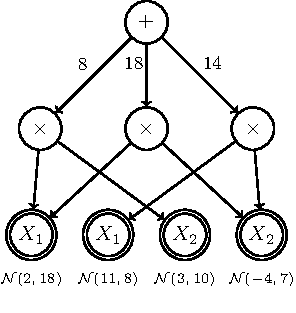
\includegraphics{figures/gspn-a.pdf}
    }

    (a)
  \end{minipage}\begin{minipage}{0.31\textwidth}
    \centering
    \scalebox{0.8}{
      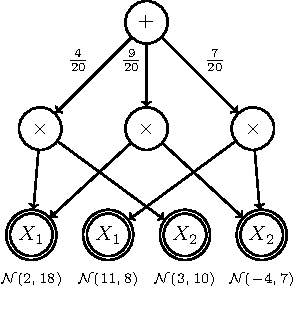
\includegraphics{figures/gspn-b.pdf}
    }

    (b)
  \end{minipage}\begin{minipage}{0.38\textwidth}
    \centering
    \scalebox{0.68}{
      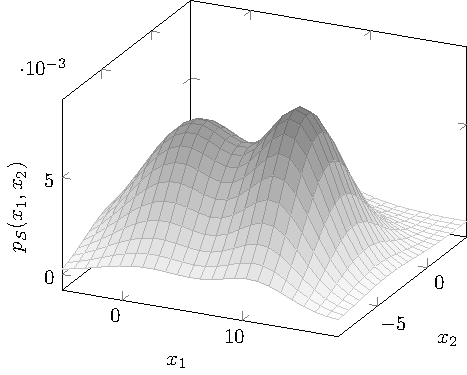
\includegraphics{figures/gspn-c.pdf}
    }

    (c)
  \end{minipage}

  \caption{
    \textbf{(a)} An unnormalized GSPN $\mathcal{S}$.
    \textbf{(b)} A normal SPN $\mathcal{S'}$ representing the same distribution of $\mathcal{S}$.
    \textbf{(c)} Plot of the PDF of $\mathcal{S}$.
  }
  \label{fig:gspn}
\end{figure}

A \emph{Gaussian Sum-Product Network (GSPN)} is a SPN in which all leaves are univariate Gaussian distributions. Figure \ref{fig:gspn} shows a representation of an unnormalized GSPN in (a), a normal GSPN representing the same distribution of it in (b), and a plot of the probability density function (PDF) of the distribution in (c).

\subsection{Induced trees and Gaussian Mixture Models}
\label{subsec:mixtures}

By definition, SPNs represent mixture distributions. \cite{Zhao2016} showed that any SPN is equivalent to a mixture of trees where each tree corresponds to a product of univariate distributions.

Given an SPN $\mathcal{S}$ over $X_1, \cdots, X_n$, let $\mathcal{T} = (V_\mathcal{T}, E_\mathcal{T})$ be a subgraph of $\mathcal{S}$. $\mathcal{T}$ is called an \emph{induced tree}
%\footnote{This concept has been used in the literature under different terms: \emph{induced tree} in \cite{Zhao2016}, \emph{parse tree} in \cite{Mei2017}, \emph{complete subnetwork} in \cite{Desana2016}, \emph{complete sub-circuit} in \cite{Chan2006} and \cite{Dennis2015}.}
from $\mathcal{S}$ if it can be constructed recursively, starting from the root node and then including all children of product nodes and exactly one child of sum nodes (with the corresponding edges). As proved by \cite{Zhao2016}, an induced tree $\mathcal{T}$ is an SPN, therefore $\mathcal{T}(\mathbf{X})$ represents a probability distribution. The density function of such distribution is given by:
\begin{equation}
  \mathcal{T}(\mathbf{x}) = \prod_{(u, v) \in E_\mathcal{T}} w(u, v) \prod_{j=1}^{n} T_j(x_j),
  \label{eq:inducedtree}
\end{equation}
where $w(u, v)$ is the weight of the edge $(u, v) \in E_\mathcal{T}$ if $u$ is a sum node or $1$ if $u$ is a product node; $T_j(X_j)$ is the probability distribution of a leaf of $\mathcal{T}$ (note that $\mathcal{T}$ contains $n$ leaves, one for each variable).

\begin{figure}
  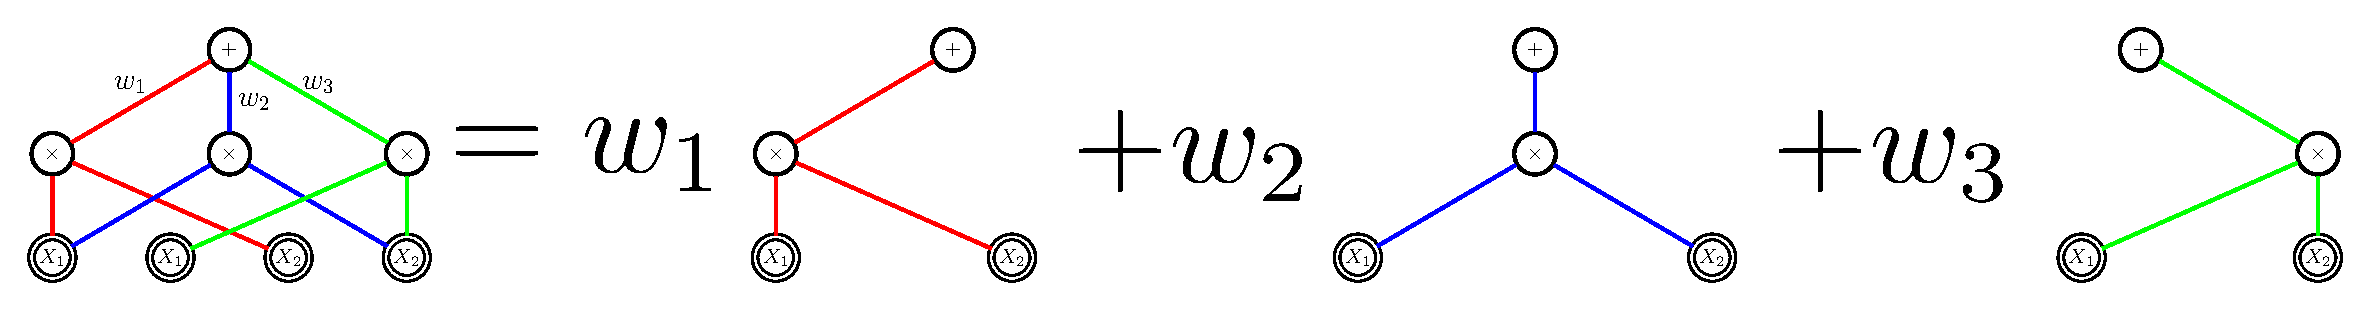
\includegraphics[width=\textwidth]{figures/inducedtrees.pdf}

  \caption{An SPN as a mixture of induced trees. Source: \cite{Zhao2016}.}
  \label{fig:inducedtrees}
\end{figure}

Let $\tau_\mathcal{S}$ denote the number of unique induced trees from $\mathcal{S}$, namely, its \emph{network cardinality}, and $\mathcal{T}^i$ denote the $i$-th unique induced tree of $\mathcal{S}$. Then \cite{Zhao2016},
\begin{equation}
  \mathcal{S}(\mathbf{x}) = \sum_{i=1}^{\tau_\mathcal{S}} \mathcal{T}^i(\mathbf{x}).
  \label{eq:mixture}
\end{equation}
This result is illustrated in Figure \ref{fig:inducedtrees}. The network cardinality of $\mathcal{S}$ depends on its structure and is exponential in the height of the SPN.
Given an SPN $\mathcal{S}$, from equations \ref{eq:inducedtree} and \ref{eq:mixture} we have:
\begin{equation}
  \mathcal{S}(\mathbf{x}) = \sum_{i=1}^{\tau_\mathcal{S}} w_i T^i(\textbf{x}),
\end{equation}
where $w_i := \prod_{(u, v) \in E_{\mathcal{T}_i}} w(u, v)$ and $T^i(\mathbf{x}) := \prod_{j=1}^n T^i_j(x_j)$ for all $i = 1, \cdots, \tau_\mathcal{S}$ (we are just splitting $\mathcal{T}_i$).

Let $Z$ be the latent variable that corresponds to the mixture, i.e., $\mathcal{S}(\mathbf{x} \mid z) = T^z(\textbf{x})$, and let $x_k, \cdots, x_l$ be values of RVs in $\mathbf{X}$. Then, for all $z \sim Z$, we have that
\begin{equation}
  \mathcal{S}(x_k, \cdots, x_l \mid z)  =  T^z(x_k, \cdots, x_l) 
  =  T^z_k(x_k) \cdots T^z_l(x_l) %\\
   =  \mathcal{S}(x_k \mid z) \cdots \mathcal{S}(x_l \mid z),
\end{equation}
which implies that the (observable) variables are independent given the mixture.
If $\mathcal{S}$ is a GSPN, then $T^z(\mathbf{X})$ is a PDF formed by the product of the PDFs of independent Gaussian RVs. Thus, $T^z(\mathbf{X})$ is a multivariate Gaussian distribution with a diagonal covariance matrix. Therefore, a GSPN represents a GMM, where in each component the variables are uncorrelated.
%
However, GSPNs have an exponential network cardinality (with respect to the height of the network); therefore, they represent GMMs with a huge number of components, which makes them much more expressive than the usual learned GMMs while still tractable.

\section{Finding the Modes of Gaussian Sum-Product Networks}
\label{sec:modes}

The problem of finding global or local maxima of a density function has been studied since long before the introduction of SPNs. The most common approach to solve it is performing hill-climbing algorithms \cite{Russell2010, Carreira-Perpinan2000}.

The density function we would like to maximize is an exponential mixture of multivariate Gaussian distributions, as shown in Section \ref{sec:spn}. \cite{Carreira-Perpinan2003, Carreira-Perpinan2003a} analyzed the number of modes of Gaussian mixtures and demonstrated that the number of modes can exceed the number of components of mixtures. That means that GSPNs can have an exponential number of modes, so finding the global optimum by local search would require a large number of restarts.
%
\cite{Amendola2019} argued that it is not known whether the number of modes is finite for general Gaussian mixtures. In the case of a finite number of modes, they proved an upper bound for the number of modes of a mixture of $k$ Gaussians with $n$ variables that is exponential in $k$ and $n$: $2^{n+\binom{k}{2}}(5+3n)^k$. Thus, GSPNs can have over exponentially many modes on their size.

\subsection{Modal EM}
\label{subsec:mem}

Investigating clustering of mixtures, \cite{Li2007} introduced a hill-climbing method named \emph{Modal EM} that solves a local maximum of a mixture density by ascending iterations starting from any initial point. It has some advantages over other existing methods such as being proved, ascending and very quick.
%
Given a mixture density of $\tau$ components $p(\mathbf{x}) = \sum_k^\tau w_k p^k(\mathbf{x})$ and an initial value $\mathbf{x}^{(0)}$, Modal EM finds a local maximum of the mixture by alternating the following two steps (starting with $r = 0$):

%\begin{enumerate}
%  \item 
%\noindent\emph{Expectation:} Let
        \begin{equation}
        \text{\textbf{Expectation}: Let }
          q_k = \frac{w_k p^k(\mathbf{x}^{(r)})}{p(\mathbf{x}^{(r)})},
          \text{ for } k = 1, \cdots, \tau.
        \end{equation}

%  \item 
%\noindent\emph{Maximization:} Update
        \begin{equation}
        \text{\textbf{Maximization}: Compute }
          \mathbf{x}^{(r+1)} = \arg\max_\mathbf{x} \sum_k^\tau q_k \log p^k(\mathbf{x}).
        \end{equation}
%\end{enumerate}

In this work, we adapt that method to create an algorithm for efficiently computing a local maximum of the mixture represented by a GSPN. Each iteration of the algorithm takes $\Theta(n |\mathcal{S}|)$ where $n$ is the number of random variables and $|\mathcal{S}|$ is the number of nodes in the GSPN. The network is traversed from the bottom up and each node propagates $2n$ values. The algorithm pseudo-code is shown in Algorithm \ref{alg:mem}.

\begin{algorithm}[h]
\caption{Modal EM for GSPNs}
\label{alg:mem}
\begin{algorithmic}
    \Input{$\mathbf{x}^r$}
    \Output{$\mathbf{x}^{(r+1)}$}
    \ForAll{node $v$ in reverse topological order}
        \If{$v$ is a leaf}
            \LineComment{Let $y$ be the RV in the scope of $v$;
            let $\mu$ and $\sigma$ be the parameters of the Gaussian of $v$;
            let $v(z)$ be the value of the Gaussian of $v$ at $z$.}
            \State $N^v_y \gets \frac{v(x^r_y)\mu}{\sigma^2}$,  $D^v_y \gets \frac{v(x^r_y)}{\sigma^2}$
            \ForAll{RV $z \neq y$}
                \State $N^v_z \gets D^v_z \gets v(x^r_y)$
            \EndFor
        \ElsIf{$v$ is a product node}
            \ForAll{RV $z$}
                \State $N^v_z \gets \prod_{c \in \ch(v)} N^c_z$
                \State $D^v_z \gets \prod_{c \in \ch(v)} D^c_z$
            \EndFor
        \ElsIf{$v$ is a sum node}
            \ForAll{RV $z$}
                \State $N^v_z \gets \sum_{c \in \ch(v)} w(v, c) N^c_z$
                \State $D^v_z \gets \sum_{c \in \ch(v)} w(v, c) D^c_z$
            \EndFor
        \EndIf
    \EndFor
    \State \Return{$\frac{N^{root}}{D^{root}}$}
\end{algorithmic}
\end{algorithm}

We show next that this algorithm performs Modal EM in a GSPN by construction. 
If $S(\mathbf{x})$ is the density of a GSPN, then $T^k(\mathbf{x})$ ($k = 1, \cdots, \tau$) corresponds to the multiplication of the densities in the leaves of its $k$-th induced tree, as seen in Subsection \ref{subsec:mixtures}. Let $T^k_i(x_i)$ the density of the leaf with scope $i$, $X_i \sim \mathcal{N}(\mu_{k_i}, \sigma^2_{k_i})$, in the $k$-th induced tree. Then:
\begin{equation}
  T^k(\mathbf{x}) = \prod_i^n T^k_i(x_i) \, ,
\end{equation}
where $n$ is the number of RVs in the SPN. Therefore,
\begin{eqnarray}
  x^{(r+1)} & = & \arg\max_\mathbf{x} \sum_k q_k \left( \log{\prod_i T^k_i(x_i)} \right) \\
  & = & \arg\max_\mathbf{x} \sum_k q_k \left(\sum_i \log{T^k_i(x_i)} \right) \\
  & = & \arg\max_\mathbf{x} \sum_k \sum_i \left(q_k \log{T^k_i(x_i)} \right) \\
  & = & \times_i \arg\max_{x_i} \sum_k \left(q_k \log{T^k_i(x_i)} \right).
\end{eqnarray}
The last equation above states that each coordinate of the $x^{(r+1)}$ vector is obtained separately, by maximizing only over the corresponding dimension $x^{(r+1)}_i$.
Hence, for a fixed $i$, we only need to find $x_i$ that maximizes $g(x_i) := \sum_k q_k \log{T^k_i(x_i)}$.

The logarithm of the probability density function $f(x)$ of a Gaussian univariate distribution with mean $\mu$ and variance $\sigma^2$ is:

\begin{equation}
  l(x) = \log{f(x)} = -\log(\sigma) - \frac{1}{2} \log(2\pi) - \frac{(x-\mu)^2}{2\sigma^2}.
\end{equation}

The first and second derivatives of that function are, respectively:

\begin{equation}
  l'(x)  =  \frac{\mu - x}{\sigma^2}, \text{ and }
  l''(x)  =  -\frac{1}{\sigma^2}.
\end{equation}

\noindent That implies that $g(x_i)$ is a sum of quadratic functions with negative second derivative, therefore it has exactly one maximum. Its derivative is:

\begin{equation}
  g'(x_i) = \sum_k^\tau \left( q_k \frac{\mu_{k_i} - x_i}{\sigma_{k_i}^2} \right) \, .
\end{equation}

\noindent Thus, to compute $x^{(r+1)}_i = \arg\max_{x_i} g(x_i)$ we can calculate the point where it is zero. By solving $g'(x_i) = 0$ we get:

\begin{equation} \label{eq:memfraction}
  x^{(r+1)}_i = \frac{\sum_k^\tau \frac{q_k \mu_{k_i}}{\sigma_{k_i}^2}}{\sum_k^\tau \frac{q_k}{\sigma_{k_i}^2}} 
  = \frac{\sum_k^\tau \frac{w_k T^k(\mathbf{x}^{(r)}) \mu_{k_i}}{\mathcal{S}(\mathbf{x}^{(r)}) \sigma_{k_i}^2}}{\sum_k^\tau \frac{w_k T^k(\mathbf{x}^{(r)})}{\mathcal{S}(\mathbf{x}^{(r)}) \sigma_{k_i}^2}} 
   =   \frac{\sum_k^\tau \frac{\mu_{k_i}}{\sigma_{k_i}^2} w_k T^k(\mathbf{x}^{(r)})}{\sum_k^\tau \frac{1}{\sigma_{k_i}^2} w_k T^k(\mathbf{x}^{(r)})}. 
\end{equation}

That is the value, for each $i = 1, \cdots, n$, that we want to compute efficiently using the GSPN. Note that the numerator and the denominator of the fraction in Equation \ref{eq:memfraction} are very similar to the evaluation of the GSPN in $\mathbf{x}^{(r)}$, $\mathcal{S}(\mathbf{x}^{(r)}) = \sum_k^\tau w_k T^k(\mathbf{x}^{(r)})$, but there is a constant (based in the parameters of the leaf of the RV $i$ in the $k$-th induced tree) multiplying $w_k$ in both cases; for the numerator, $\frac{\mu_{k_i}}{\sigma^2_{k_i}}$, and for the denominator, $\frac{1}{\sigma^2_{k_i}}$.

That is why our algorithm performs a bottom-up evaluation of the GSPN propagating $2n$ values for each node: for each RV, one to compute the numerator ($N$) and the other for computing the denominator ($D$) of the Equation \ref{eq:memfraction}. In the end, we just divide the vectors ($N$ by $D$) to get $\mathbf{x}^{(r+1)}$.

Our implementation of Modal EM for GSPNs is released as open source in the RPCircuits.jl Julia package for learning and inference with  SPNs.\footnote{Available at \url{https://github.com/RenatoGeh/RPCircuits.jl}.}

\section{Applications}
\label{sec:experiments}

In this section we discuss some potential  applications of computing the modes of GSPNs in Maximum-A-Posteriori (MAP) Inference and hierarchical clustering. 
As our intention here is not to establish state-of-the-art solutions for these tasks, we leave empirical comparisons with competing methods as future work.

\subsection{Maximum-A-Posteriori inference}
\label{subsec:map}

SPNs are often build to solve structured prediction problems, where a structure solution is found by Maximum-A-Posteriori (MAP) inference in the model, that is, by searching for the most probable values for a set of RVs according to a probability distribution or for the global maximum configuration of the probability density function\footnote{Strictly, MAP problem considers three disjoint sets $\mathbf{X}^q$, $\mathbf{X}^0$ and $\mathbf{X}^m$ such that $\mathbf{X} = \mathbf{X}^q \cup \mathbf{X}^0 \cup \mathbf{X}^m$ and consists in finding the most probable configuration for $\mathbf{X}^q$ given an evidence $\mathbf{x}^0$ on variables $\mathbf{X}^0$ and ignoring (marginalizing) the RVs in $\mathbf{X}^m$. However, \cite{Mei2017} proved that, for SPNs, every such problem can be reduced to a special case of MAP inference without evidence and RVs to marginalize in linear time in the size of the network. That is why we can say it consists in simply finding the global maximum of a probability density function.}. MAP inference is useful for many tasks, especially in applications that require reconstructing data such as image completion. Since the problem is $\mathcal{NP}$-Hard in SPNs \cite{Peharz2015, Peharz2016, Conaty2017}, different greedy approximation algorithms have been proposed: the first was Max-Product \cite{Poon2011} and then some variations of it such as Beam Search \cite{Park2002}, ArgMax-Product \cite{Conaty2017}, and K-Best Tree \cite{Mei2017}. \cite{Mei2017} also proposed an exact algorithm that performs an exhaustive search in the space of solutions with a combination of pruning, heuristic and optimization techniques. More recently, \cite{Maua2020} proposed two reformulation approaches to MAP inference in SPNs: one casting the problem as a similar inference in Bayesian networks and other casting it as a mixed-integer linear programming for which there exists efficient solvers.

The above mentioned works focus on discrete SPNs (although some are easily extensible to continuous domains) and do not report experiments with continuous data; most importantly, they usually search only the limited space of modes of the distributions at the leaves and thus deliver solutions of unknown quality, which are unable to ensure even local optimality (i.e., they do not necessarily find a mode of the joint density). To see why searching over the modes of the leaves might fail at finding a local maximal, consider the simple univariate GSPN in Figure~\ref{fig:shortcomings}, shown as a circuit and the respective density.
As can be seen from the left plot, the maximum of the density occurs at $X = 2$ ($p(2) \approx 0.125$). However, greedy algorithms such as MaxProduct~\cite{Poon2011} and K-Best Tree~\cite{Mei2017} find either solutions $X = 1$ or $X = 3$ ($p(1) = p(3) \approx 0.119$).

\begin{figure}
  \begin{minipage}{0.5\textwidth}
    \centering
    \scalebox{0.55}{
      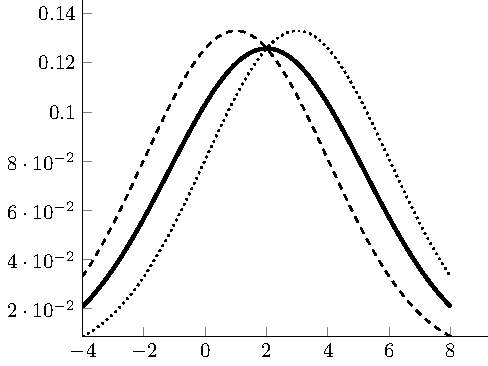
\includegraphics{figures/shortcomings-a.pdf}
    }

    (a)
  \end{minipage}\begin{minipage}{0.5\textwidth}
    \centering
    \scalebox{1.1}{
      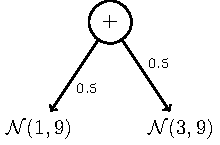
\includegraphics{figures/shortcomings-b.pdf}
    }

    (b)
  \end{minipage}

  \caption{
    \textbf{(a)} Plot of the PDFs of three distributions: $X \sim \mathcal{N}(1, 9)$ (dashed line); $X \sim \mathcal{N}(3, 9)$ (dotted line); $X \sim 0.5 \mathcal{N}(1, 9) + 0.5 \mathcal{N}{3, 9}$ (solid line).
    \textbf{(b)} GSPN representing the univariate GMM $X \sim 0.5 \mathcal{N}(1, 9) + 0.5 \mathcal{N}(3, 9)$. The existing algorithms are unable to find its optimal MAP, $X = 2$.
  }
  \label{fig:shortcomings}
\end{figure}

We can use the Modal EM algorithm to improve MAP solutions as follows. 
First, Modal EM can be run starting with the solution found by any earlier mentioned algorithm. That way we can guarantee that we are finding a stationary point; in the previous univariate GSPN example, that would result in us finding the optimal MAP. Second, we can run Modal EM from several input data points (e.g., a subsample of the training data set) to find different modes of the density function; then we can compare their likelihoods and pick the maximum. 
That is similar to the one of the methods proposed in \cite{julissa-bracis} for discrete SPNs. 
Note that such an approach improves on any given MAP Inference algorithm for GSPNs with only a small overhead.

\subsection{Hierarchical clustering}
\label{subsec:clustering}

\cite{Li2007} proposed using Modal EM in  Gaussian Mixture Models as a way to perform semi-parametric clustering. Their approach is to consider that a cluster is formed by the instances that ascend to the same mode of the density function. Modes are arguably good representatives of clusters, since each of them correspond to the local maximum of all points of a cluster. Since there are many modes in Gaussian mixtures, this method is extended for hierarchical clustering by recursively learning models from the modes found in the previous iterations. In their work, they use kernel density estimators with increasing bandwidths.

As an illustrative example of extending such an idea to GSPNs, which arguably capture a more flexible and expressive class of statistical models, we show empirical results of iteratively learning new GSPNs from the modes found by Modal EM in the previously model. That way we iteratively learn simpler and smaller models using the modes of the previously learned models, which arguably provide a representative summary of the data and model. This is therefore connected to two applications: hierarchical semi-parametric clustering and model compression.

We use the classical MNIST database of handwritten digits. The dataset contains 60,000 28x28 grayscale images of the 10 digits (0--9) in the training set and 10,000 images in the test set. Each of the 784 pixels contain an integer value ranging from 0 to 255. We considered only the images of the digit 0 from the MNIST database. In such a subset, which we will call MNIST-0, there are 5,923 images in the training set and 980 images in the test set.

\begin{table}
    \centering
    \caption{SPNs learned from MNIST-0 training set at iteration 1 and modes found in the first iteration at iteration 2. For each iteration, the tables show the number of instances used to learn the model, the network size (given by the number of nodes in the SPN), the number of clusters as found by running Modal EM starting from every point in the training set, and the log of the average likelihood for the test set in the learned SPN.}
    \label{tab:experiments}
    \begin{tabular}{|c|r|r|r|r|}
        \hline
        \textbf{Iteration} & \textbf{\# Instances} & \textbf{Network size} & \textbf{\# Clusters} & \textbf{Log Avg. Likelihood} \\ \hline
        \textbf{1} & 5,923 & 74,556 & 201 & ~7,707 \\
        \textbf{2} & 201 & 7,851 & 10 & ~3,438 \\
        \hline
    \end{tabular}
\end{table}

We learned a sequence of GSPNs using the LearnSPN implementation in open-source Python library SPFlow \cite{Molina2019SPFlow},\footnote{Available at \url{https://github.com/SPFlow/SPFlow}.} as follows.
We first learn an initial GSPN from the MNIST-0 dataset, and use our Modal EM algorithm with each datapoint in the training set to obtain a set of representative summaries (modes).
Points that ``converge'' to the same mode are assigned to the same clustering.
The set of modes obtained form a new dataset, from which we learn a new GSPN and the process repeats until the number of modes is sufficiently small.
In our experiments, two iterations sufficed to obtain a small set of models/clusters.

The results are shown in Table \ref{tab:experiments}. 
We report the size of the network and the log of the average likelihood of the test set in the learned SPN. That way we can see how good the model is to represent the examples in the test set. Figure \ref{fig:clusters} shows the hierarchical clustering obtained by the process for the MNIST-0 dataset. For clarity, we omit the initial 5,923 instances of the training dataset, and show only the modes found by Modal EM in the first and second iterations. 
Even in a network with about 10\% of the size of the original network, the modes appear to be  good representatives of the diversity of the dataset.


\begin{figure}
    \centering
    \scalebox{0.19}{
        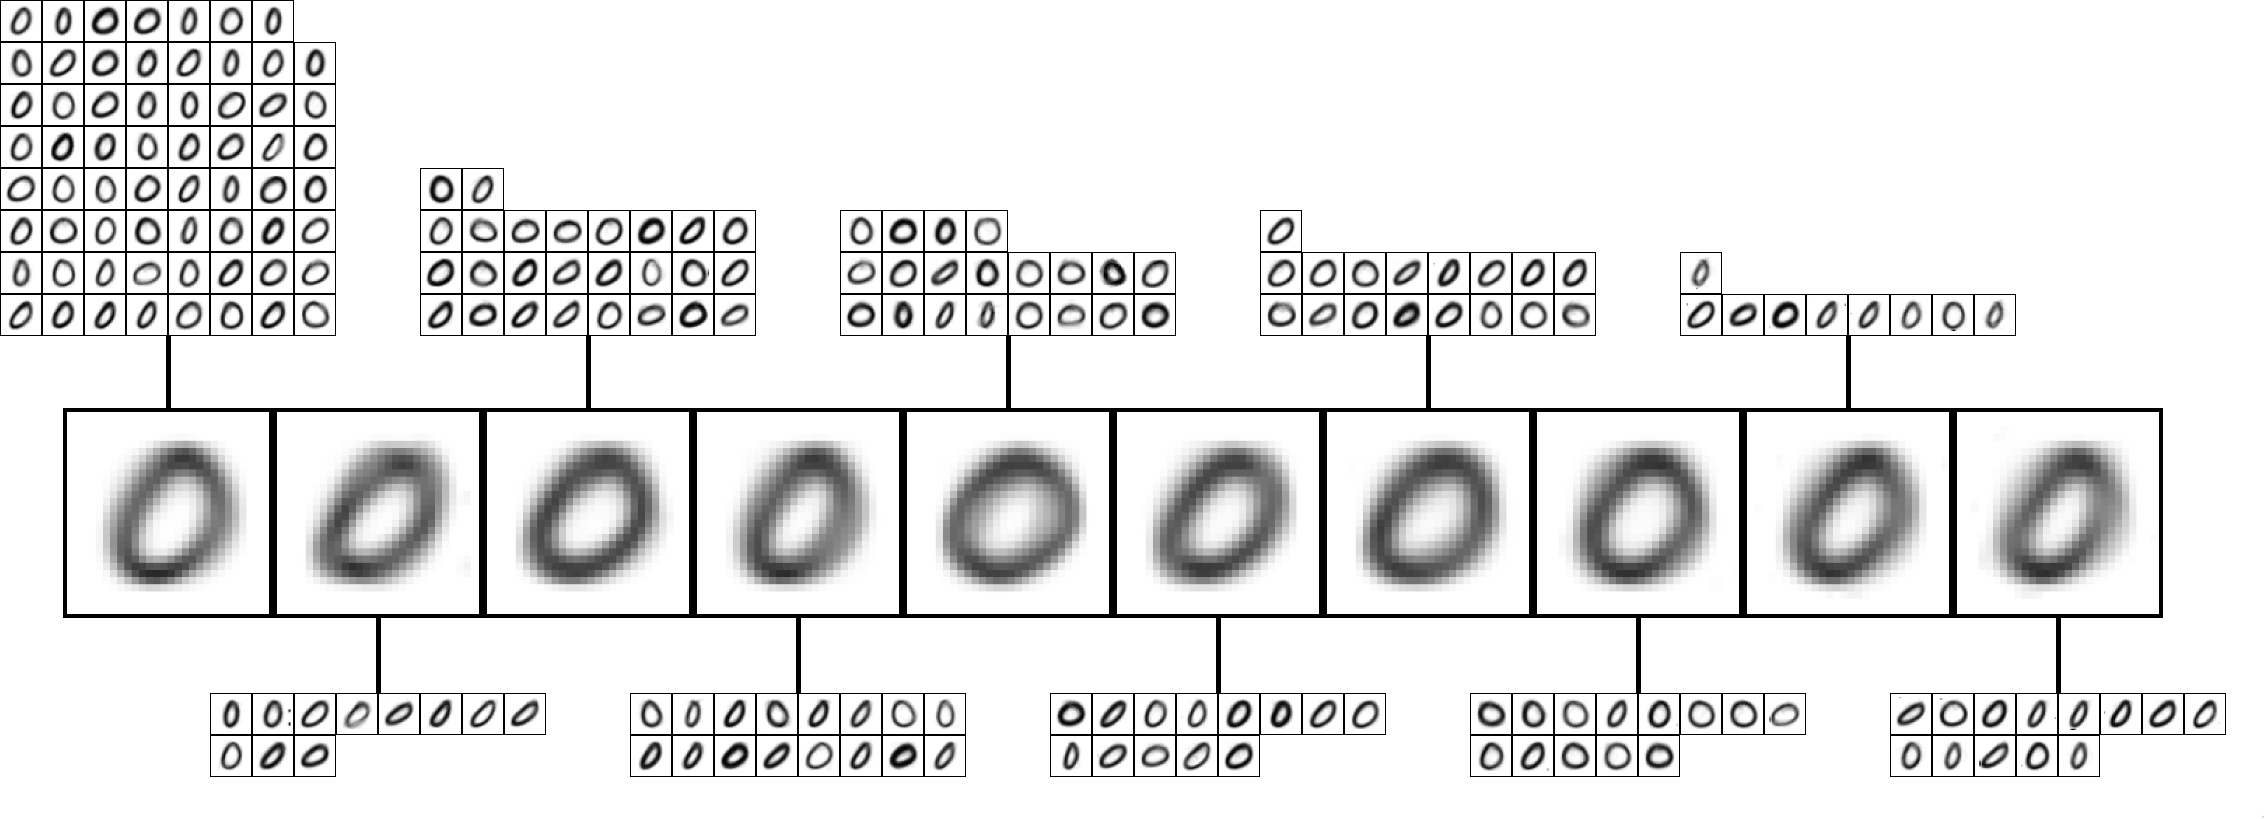
\includegraphics{figures/clusters.png}
    }
    \caption{Hierarchical clustering: Modes (representatives of the clusters) found in 2 iterations of Modal EM in GSPNs learned from MNIST-0 dataset. The smaller images correspond to the modes found in the first GSPN, the bigger ones correspond to the modes found in the second GSPN (learned from the modes from the first GSPN). Modes from the first GSPN are connected to their modes in the second GSPN.}
    \label{fig:clusters}
\end{figure}

One drawback of such an approach is that high density regions (or equivalent, large cluster) are underrepresented in the new dataset, while low density regions (small cluster) are overrepresented.
We could mitigate such issues by optimizing for weighted log-likelihood in the structural and parametric learning algorithms, or more simply by over/undersampling models according to the respective region's density.
We leave for future work an empirical comparison of such ideas.

\section{Conclusions and future work}
\label{sec:conclusion}

Sum-Product Networks (SPNs) are a class of statistical models that generalize Finite Mixture Models while retaining nice computational properties such as linear-time marginal inference and parameter learning.
As with Finite Mixture Models, finding the modes of such densities remains a challenging problem.

Based on previous work on Gaussian Mixture Models, in this work we developed a linear-time algorithm for finding the local maxima of a joint density distribution described as a Sum-Product-Network with Gaussian leaves.
To our knowledge, the proposed algorithm, Model EM (named from its relation to Expectation-Maximization approach of latent variable models), is the first work specially desgined to address the problem of finding modes in continuous Sum-Product-Networks.

After developing the algorithm and analysing the correctness and time efficiency of the algorithm, we discuss some practical applications of mode finding in performing MAP inference,  hierarchical clustering and data/model compression.
For MAP inference, we argued that Modal EM can be used to improve the solution of any existing algorithm, leading to an algorithm which provably finds local optimal (a property most current algorithms lack).
For hierarchical clustering, we performed an illustrative experiment with images of the digit zero from the MNIST dataset that described how the approach can be used to categorize, explore or compress data.

We leave as future work a more extensive empirical comparison of Modal EM in such applications.
Another avenue to explore in future work is the use of Modal EM for discrete SPNs.
In principle, we can treat Bernoulli leaves in discrete Sum-Product-Networks as continuous variables and apply the same formulas to derive an approximate algorithm for local maximizers of the joint distributions.
The solutions obtained by the algorithm then can be either rounded or fed into another algorithm to obtain valid solutions.


\section*{Acknowledgments}

This work was partly supported by the FAPESP-IBM grant \#2019/07665-4 and CNPq PQ grant \#304012/2019-0.

\bibliographystyle{sbc}
\bibliography{references}

\end{document}
